\label{chap:implementation}
In this chapter, we discuss our implementation of CAL. We used this
implementation to perform all the experiments described in the future chapters.
We start by reviewing the original implementation of CAL, followed by our goals
and expectations from the new implementation. We then briefly discuss the
design decisions, along with the capabilities of our system.

The code for our system is open source and available with documentation
online\footnote{\url{https://hical.github.io/}}.

\section{Auto-TAR BMI}
As mentioned in the previous chapter,
BMI\footnote{\url{https://plg.uwaterloo.ca/~gvcormac/trecvm/}} (Baseline Model
Implementation) is an implementation of CAL which was used as a baseline in the
TREC 2015 and 2016 Total Recall track. Most of BMI is written as
a BASH script, which coordinates various external programs to perform more
more specific tasks like training and scoring. Most of the intermediate data is
stored in text files since BASH is not designed to support advanced data
structures.

\section{CAL++}

\subsection{Motivation and Goals}
For the refresh strategy defined in BMI, the BASH system works reasonably well.
However, its inefficiencies become more significant as we design refresh
strategies which require more computation. While the original
implementation is suitable for simulation purposes, it is inefficient and
difficult to use in real world applications.

As part of our TREC 2017 Core effort, we designed a CAL-powered review tool
called HiCAL. We intended this tool to process relevance feedback as quickly as
possible (in other words, more frequent refreshes). For a smooth user
experience, we wanted to achieve this with minimum possible system delay. Due to
to these reasons, we decided to implement CAL from scratch in C++. We chose C++
because it provides a good control over efficiency and is usually easy to
maintain/extend.

We wanted to build a system which along with satisfying all the requirements of
HiCAL, could be easily used for other applications and future research, such as
the work presented in this thesis. We designed this system to meet the following
goals:

\begin{itemize}
\item Fast and efficient.
\item Support parallel tasks (for parallel simulations and multiple users).
\item Easy to use as a standalone tool or as a part of an external application.
\item Easy to extend and modify any step of the CAL algorithm.
\end{itemize}

\subsection{Design}
In this section, we briefly discuss the design details of our CAL system.

Prior to using the CAL system, a one-time preprocessing step is required to convert a
given text collection to a machine readable set of feature vectors. The corpus
processor takes as input an archive (a tar.gz file) of text documents, computes
the feature vectors for every document, and writes them to a binary file. We use
binary files over human-readable text files to significantly improve the output
file size and loading times. \red{Provide numbers to quantify the difference}
Each document is assigned an ID which is its base filename in the input archive
(filename ignoring the directory structure). This ID is used to judge and
retrieve documents in the CAL system. The files are treated as plaintext files
and are assumed to be cleaned as per the needs of the user.
Figure~\ref{fig:preprocessing} shows a preprocessing pipeline example with New
York Times collection.  By default, the corpus preprocessor computes tf-idf
unigram features for every documents as explained in the previous chapter.

\begin{figure}[h]
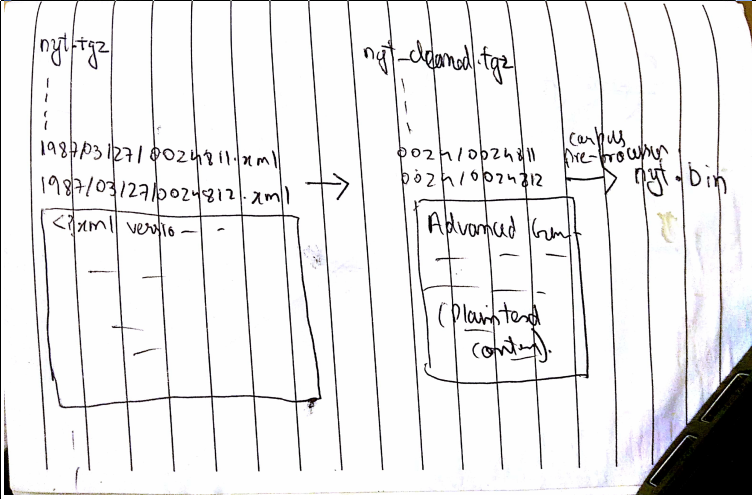
\includegraphics[width=\textwidth]{tmp_pictures/preprocessing_pipeline.png}
\caption{Preprocessing pipeline for New York Times collection}
\label{fig:preprocessing}
\end{figure}

The output binary file contains document frequency data followed by the document
feature data. The binary file format is described in
Figure~\ref{fig:binary_format}.

\begin{figure}[h]
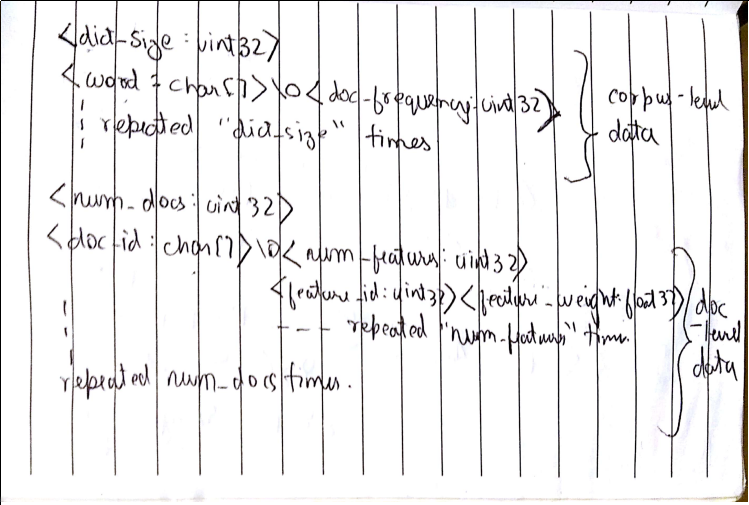
\includegraphics[width=\textwidth]{tmp_pictures/binary.png}
\caption{Description of the binary file outputted by the corpus preprocessor}
\label{fig:binary_format}
\end{figure}

The CAL system takes as input the corpus features (the binary output file of the
corpus preprocessor) and loads it in the memory. The document feature vectors
are kept in the memory throughout the lifetime of a CAL process in order to
ensure fast operations and reduce disk access. A review task is initiated by a
seed query string provided by the user. The user can also specify seed document
judgments and the choice of refresh strategy at the beginning of a task. The
system handles these tasks concurrently, so that multiple users can review
documents at the same time.

Training and scoring all the documents constitute majority of the computation.
For training, we modified sofia-ml so that we can invoke its functions natively
through our code and make it compatible with our data structures. We also
stripped away unneeded parts from the sofia-ml source code. The weight vector
obtained from training is used to fetch few top documents from a set (depending
on the refresh strategy). The score for a single document is calculated by
performing an inner product of the document feature vector with the trained
weight vector. The scoring of all the documents is parallelized across multiple
threads (8 by default).

The CAL system is designed such that it is easy to extend or modify parts of the
algorithm. Most of the refresh strategies mentioned in this thesis were
implemented by extending a class and overriding few methods.

There are multiple ways to interact with the CAL system. The robust and user-friendly
HTTP API should be used for most purposes. Python bindings for the CAL system is
also available (it is an abstraction over the HTTP API). The command line tool
can be used for testing and simulation purposes.
